\documentclass[tikz,convert,convert={command=\unexpanded{
  call ./util/mk_folder out_png
  && cd /d out_png
  && call ../util/pdf_to_png.bat 600 ../\infile\space \outfile\space
}}]{standalone}
\usepackage{tikz}
\usetikzlibrary{intersections}
\tikzset{help lines/.style=very thin}
\tikzset{Karl's grid/.style={help lines,color=blue!50}}
\begin{document}
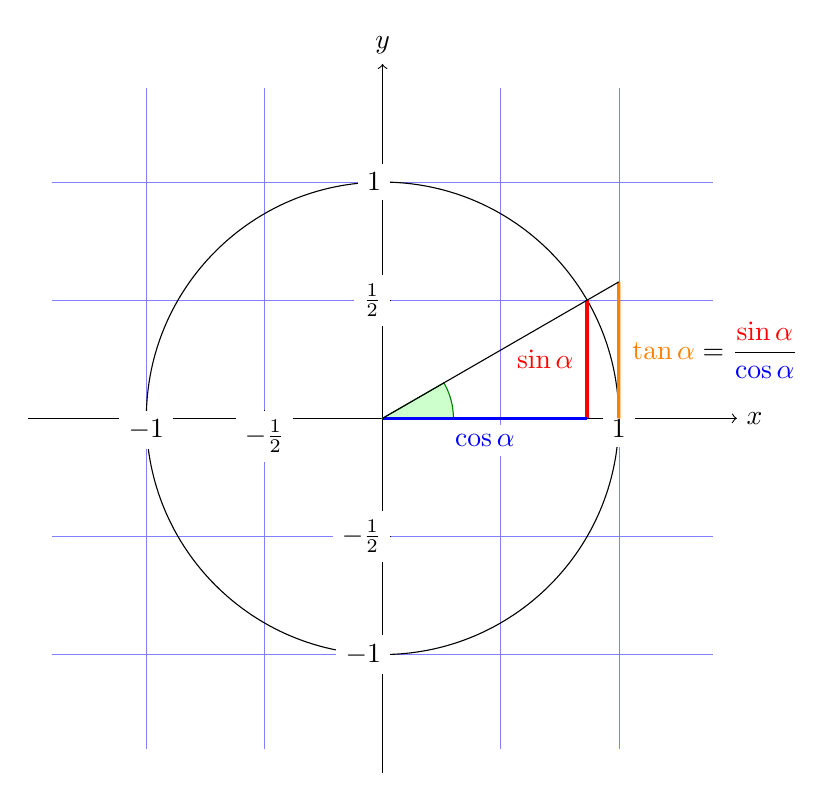
\begin{tikzpicture}[scale=3]
    
    %\clip (-2,-0.2) rectangle (2,0.8);
    \draw [step=.5cm,Karl's grid]  (-1.4,-1.4) grid (1.4,1.4);
    \draw[->]  (-1.5,0) -- (1.5,0) node[right] {$x$} coordinate (x axis);
    \draw[->]  (0,-1.5) -- (0,1.5) node[above] {$y$} coordinate (y axis);
    \draw  (0,0) circle [radius=1cm];
    \filldraw[fill=green!20!white,draw=green!50!black] (0,0) -- (3mm,0mm)
          arc [start angle=0, end angle=30, radius=3mm] -- cycle;

    \draw[red,very thick] 
      (30:1cm) -- node[left=1pt,fill=white]{$\sin \alpha$} (30:1cm |- x axis);
    \draw[blue,very thick] 
      (30:1cm |- x axis) -- node[below=2pt,fill=white]{$\cos\alpha$} (0,0);

    \foreach \x/\xtext in {-1,-0.5/-\frac{1}{2},1}
      \draw (\x cm,-1pt) -- (\x cm,1pt) node[anchor=north,fill=white] {$\xtext$};
    \foreach \y/\ytext in {-1,-0.5/-\frac{1}{2},0.5/\frac{1}{2},1}
      \draw (-1pt,\y cm) -- (1pt,\y cm) node[anchor=east,fill=white] {$\ytext$};

    \path [name path=upward line] (1,0) -- (1,1);
    \path [name path=sloped line] (0,0) -- (30:1.5cm);
    \draw [name intersections ={of=upward line and sloped line,by=t}]
          [very thick,orange] (1,0) -- node [right=1pt,fill=white] {$\displaystyle \tan \alpha \color{black}=
          \frac{{\color{red}\sin \alpha}}{\color{blue}\cos \alpha}$} (t);

    \draw (0,0) -- (t);
\end{tikzpicture}
\end{document}